\chapter{Resultados Experimentais}\label{result}

Este capítulo apresenta os resultados experimentais obtidos na indução do modelo \textit{Adaboost} sobre 30\% da base de conhecimento.

Os primeiros experimentos realizados na predição, ilustrado na Figura ~\ref{fig:resultados_experimentais_1}, demonstraram uma taxa de 40\% de acerto na predição da primeira competência exigida em um texto de redação, de uma amostra de 100 redações. 

A análise gráfica do resultado experimental demonstra que a predição do modelo está em uma faixa especifica de 0.5 a 1.5, ou seja, a indução do modelo deve ser repetida até o mesmo se tornar genérico.

\begin{figure}[H]
\begin{center}
    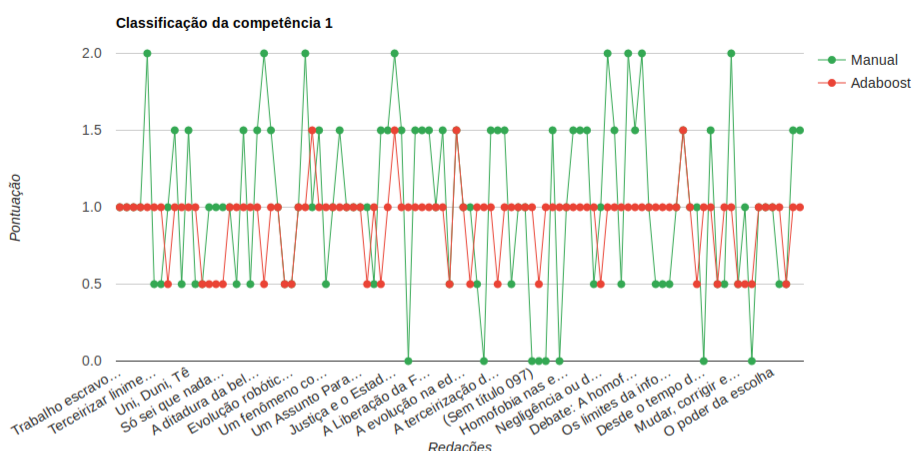
\includegraphics[scale=0.70]{figuras/resultados_experimentais.png}
\end{center}
\caption{No gráfico ilustrado os pontos verdes demosntram as redações classificadas incorretamentes pela falta de generalização do modelo induzido.}
\label{fig:resultados_experimentais_1}
\end{figure}